\chapter{Coding Approaches}

In this chapter, we will explore some low-level implementation details common to most algorithms discussed in the following chapters, as well as some important tricks and decisions made during the development of the project.

\section{Approaches to Cost Function}

In the TSP, the factor that determines whether a path in a graph is good or not is its overall cost, which represents the sum of all the edges visited along that path.
In this project, we used only instances from TSPLIB\cite{tsplib} in order to provide a wide variety of graphs for experimentation.
This section will explore three different approaches for determining the cost of each edge.

\subsection{TSPLIB Specifications}

We focused exclusively on instances where the cost of the edges in the TSP graph could be computed using specific formulas.
In these instances, each node is assigned fixed coordinates, in our case $x$ and $y$ coordinates.
Using these coordinates, the distance between each pair of nodes can be calculated using the appropriate formula according to TSPLIB specifications.
We limited ourself in the implementation of only the most popular distance functions:
\begin{itemize}
    \item EUC\_2D $round(\sqrt{(x_1 - x_2)^2 + (x_1 - x_2)^2})$
    \item MAX\_2D $round(max(|x_1 - x_2|,|x_1 - x_2|))$
    \item MAN\_2D $round(|x_1 - x_2| + |x_1 - x_2|)$
    \item CEIL\_2D $ceil(\sqrt{(x_1 - x_2)^2 + (x_1 - x_2)^2})$
    \item ATT \qquad $round(\sqrt{(x_1 - x_2)^2 + (x_1 - x_2)^2}/10)$
\end{itemize}
Where $round(k)$ returns the integer number closest to $k$ and $ceil(k)$ returns the smallest integers greater or equal than $k$.

\subsection{Basic approach}

The first and simplest method involves computing the cost each time it is needed. 
The main advantages of this approach are its inherent simplicity and its $O(2n)$ memory requirement, as it only needs to store the coordinates of the nodes in memory.
Its greatest drawback is the slow execution speed.

In the TSPLIB specifications the majority of the cost functions, which happen to be the same used during all the testing, include some computationally expensive operations.
The square root operation is one of this operations as it usually requires an iterative algorithm, like the Newton's method\cite{newtonMethod}, to be computed.
Nowadays most modern computer architectures include a hardware dedicated instructions, which can be many times faster when compared to the software conterparts, yet they still require several CPU cycles in order to be executed.
In order to use these specialized instructions some additional parameters are required when compiling the code\footnote{\textit{gcc} and \textit{clang} compilers require the parameter "-ffast-math"}.

\begin{figure}[htbp]
    \centering
    \begin{tikzpicture}
        \begin{axis}[
            width=11cm, height=8cm,
            ymajorgrids=true,
            grid style={dashed,gray!30},
            xlabel=Instance size,
            ymin=1, ymax=2,
            ylabel=,
            legend style={at={(0.02,0.98)},anchor=north west,legend columns=-1},
            symbolic x coords={100,500,1000,5000,10000},
            log ticks with fixed point,
            xtick=data,
            ytick={1,1.2,1.4,1.6,1.8,2},
            yticklabels={0\%,20\%,40\%,60\%,80\%,100\%},
            ybar, 
                    ]
            \addplot[Blue,fill] table[x=n, y=cmpbase_hwinstructions, col sep=semicolon] {csv/cmp_2opt.csv};
        \end{axis}
    \end{tikzpicture}
    \caption{Speedup of hardware specialized instructions with the Base approach in 2Opt.} \label{fig:baseHWSpecific}
\end{figure}

Another time-critical operation in the cost functions is the step in which the value is converted to integer, namely the $round$ and $ceil$ functions.
Although not presenting a slowdown as great as the square root operation, they are still executed in more than a cycle.
As with the previous case, modern computer architectures provide specific instructions which improve yet again the overall speed of this approach.
Even with all the optimization described above implemented, this approach remains the slowest one, as we will see in the comparision section.

\subsection{Cost-Matrix approach}

The Cost-Matrix approach consists in storing the cost of the edges of the graph in a matrix $A$ of size $n^2$, where each element $a_{i,j}$ represents the cost of edge $e_{i,j}$.
In this method, the costs are computed just once at the start of the execution.
Once the matrix $A$ is initialized, the cost of any edge in the graph can be accessed by retrieving the corresponding value from $A$.

The main advantage of this approach is the ability to obtain the cost of all edges without the need for recalculating them, avoiding the overhead of live computation.
However, despite this significant benefit, there are some major drawbacks.

The first is memory utilization: it requires $O(n^2 + 2n)$ memory to store both the matrix and the coordinates.
It is worth noting that matrix $A$ is symmetric, and the main diagonal consists entirely of zeros, which means memory usage can be reduced to $O(n^2/2-n+2n)$.
However, this memory optimization results in a more complex method of accessing the matrix, as the direct correspondence between edges and matrix elements would be lost.

The second major drawback lies in how modern computers handle memory.
Main memory is often a significant bottleneck for most algorithms, to the extent that the time complexity of algorithms is sometimes measured by estimating the number of memory accesses performed.
To improve performance, caching was introduced.
Caching involves storing frequently accessed portions of memory in faster memory pools, improving the overall speed of memory access.
With this in mind, cache efficiency is an important factor to consider when comparing the performance of this approach to others.
The issue arises when an algorithm requires access to locations in $A$ that are neither close together nor consistent, which can significantly reduce performance.
A clear example of this can be observed in the performance difference between using row-major indexing versus column-major indexing in $A$.
This is demonstrated in \figurename{ \ref{fig:matrixBadIndex}}, in which the speed difference increases with the size of $A$, which results in lower cache efficiency in the column-major indexing.

\begin{figure}[htbp]
    \centering
    \begin{tikzpicture}
        \begin{axis}[
            width=11cm, height=8cm,
            ymajorgrids=true,
            grid style={dashed,gray!30},
            xlabel=Instance size,
            ymin=1, ymax=6,
            ylabel=,
            legend style={at={(0.02,0.98)},anchor=north west,legend columns=1},
            symbolic x coords={100,500,1000,5000,10000},
            log ticks with fixed point,
            xtick=data,
            ytick={2,3,4,5},
            yticklabels={100\%,200\%,300\%,400\%},
            ybar, 
                    ]
            \addplot[Blue,fill] table[x=n, y=cmpmatrix_rowmajor, col sep=semicolon] {csv/cmp_2opt.csv};
        \end{axis}
    \end{tikzpicture}
    \caption{Speedup of row-major indexing against column-major indexing with the Cost-Matrix approach in 2Opt.} \label{fig:matrixBadIndex}
\end{figure}

\subsection{AVX approach}

AVX (Advanced Vector Extensions)\cite{avxWikipedia} is a set of CPU instructions designed to enhance performance by enabling parallel processing of multiple data points with a single instruction.
This approach utilizes these kind of SIMD (Single Instruction Multiple Data) extensions to achieve benefits like increased speed and lower memory usage, at the cost of simplicity: AVX code is significantly more difficult to write and debug.

In simple terms, this method extends the Basic approach by computing multiple edge costs simultaneously, at roughly the same computational cost as calculating a single one.
More specifically, AVX registers are 256 bits in size and support various operations and data types. 
In this project, we chose to use 32-bit floating-point representation for both the node coordinates and the edge costs.
This allows a single AVX register to hold a vector of eight values, effectively performing eight computations simultaneously.
If higher precision is required, AVX instructions also support 64-bit double-precision floating-point numbers, but with the limitation of processing only four elements at a time, which is half the number in our implementation.

The simplicity of the code is sacrificed in several ways.
The first challenge is the need to arrange the data in a suitable manner so that the vectors loaded into the AVX registers are consistent and not scattered across memory.
A second challenge arises from handling conditional statements involving individual variables within the eight-packed vectors, which must be processed in two phases.
Other technical difficulties involve loading the final elements of an array, which can result in loading unintended variables into the register and potentially invalidating the entire computation if not handled properly.

The use of AVX paves the way for further optimizations based on approximation.
Specifically, the square root operation is optimized by using instructions that perform the \textit{approximated reciprocal square root} and \textit{approximated reciprocal} functions.
This allows an approximation of the square root function to be obtained in a significantly shorter time frame, thanks to the improved latency and throughput of these instructions.
Of course, this type of computation can only be used when minimizing or maximizing between edges or some function of them, and the final result must be verified with the more precise function.

\begin{figure}[htbp]
    \centering
    \begin{tikzpicture}
        \begin{axis}[
            width=11cm, height=8cm,
            ymajorgrids=true,
            grid style={dashed,gray!30},
            xlabel=Instance size,
            ymin=1, ymax=1.6,
            ylabel=,
            legend style={at={(0.02,0.98)},anchor=north west,legend columns=-1},
            symbolic x coords={100,500,1000,5000,10000},
            log ticks with fixed point,
            xtick=data,
            ytick={1,1.1,1.2,1.3,1.4,1.5,1.6},
            yticklabels={0\%,10\%,20\%,30\%,40\%,50\%,60\%},
            ybar, 
                    ]
            \addplot[Blue,fill] table[x=n, y=cmpavx_approx, col sep=semicolon] {csv/cmp_2opt.csv};
        \end{axis}
    \end{tikzpicture}
    \caption{Speedup of approximated edge costs with the AVX approach in 2Opt.} \label{fig:avxApprox}
\end{figure}

\subsection{Performance Comparison}

\begin{figure}[htbp]
    \centering
    \begin{tikzpicture}
        \begin{axis}[
            width=11cm, height=8cm,
            ymajorgrids=true,
            grid style={dashed,gray!30},
            xlabel=Instance size,
            ymin=0, ymax=9,
            ylabel=Relative iterations/s,
            legend style={at={(0.02,0.98)},anchor=north west,legend columns=-1},
            symbolic x coords={100,500,1000,5000,10000},
            log ticks with fixed point,
            xtick=data,
            ytick={1,2,3,4,5,6,7,8},
            % yticklabels={100\%,200\%,300\%,400\%,500\%,600\%,700\%,800\%},
            ybar, 
                    ]
            \addplot[Blue,fill] table[x=n, y=ones, col sep=semicolon] {csv/cmp_2opt.csv};
            \addplot[Red,fill] table[x=n, y=cmp_matrix, col sep=semicolon] {csv/cmp_2opt.csv};
            \addplot[Green,fill] table[x=n, y=cmp_avx, col sep=semicolon] {csv/cmp_2opt.csv};
            \legend{Basic,Matrix,AVX}
        \end{axis}
    \end{tikzpicture}
    \caption{Comparison of all three approaches in 2-Opt (measurment were taken using the best optimizations found for each approach).} \label{fig:avxShowcase}
\end{figure}

Comparing these three approaches is complex due to numerous factors.
For example, cache efficiency may be better in some TSP instances than in others, depending on how sequentially the cost matrix is accessed.
To minimize these factors as much as possible, data was gathered using multiple instance sizes, with the most common cost function (EUC\_2D).

\figurename{ \ref{fig:avxShowcase}} compares all three methods, scaled relative to the Basic approach.
As expected, the Cost-Matrix method is faster than the Basic method for smaller instances but loses its advantage as the instance size increases, likely because the Cost-Matrix becomes too large for the CPU cache.
Throughout the testing, the AVX approach consistently proved to be the fastest by a significant margin in every scenario.
However, it should be noted that the AVX method yielded unstable results on smaller instances (fewer than 100 nodes), occasionally performing slower than the Cost-Matrix method.

\section{Multithreading}

\begin{figure}[htbp]
    \centering
    \begin{tikzpicture}
        \begin{axis}[
            % title={Multithreading speedup of 2-Opt parallel implementation},
            xlabel={Number of Threads},
            ylabel={Speedup},
            xmin=1, xmax=8,
            ymin=1, ymax=8,
            xtick={1,2,3,4,5,6,7,8},%,10,12,14,16,18,20},
            ytick={1,2,3,4,5,6,7,8},%,9,10,11,12,13,14,15,16},
            legend style={at={(0.98,0.02)},anchor=south east,legend columns=1},
            ymajorgrids=true,
            xmajorgrids=true,
            grid style=dashed,
        ]
        
        \addplot[Blue,mark=square] table[x=cores, y=nn100, col sep=semicolon] {csv/MT.csv};
        \addplot[Red,mark=o] table[x=cores, y=nn1000, col sep=semicolon] {csv/MT.csv};
        \addplot[Green,mark=triangle] table[x=cores, y=nn10000, col sep=semicolon] {csv/MT.csv};
        \addlegendentry{n=100}
        \addlegendentry{n=1000}
        \addlegendentry{n=10000}
            
        \end{axis}
    \end{tikzpicture}
	\caption{Multithreading speedup of Nearest Neighbor parallel implementation.} \label{fig:multithreadNN}
\end{figure}

\begin{figure}[htbp]
    \centering
    \begin{tikzpicture}
        \begin{axis}[
            % title={Multithreading speedup of 2-Opt parallel implementation},
            xlabel={Number of Threads},
            ylabel={Speedup},
            xmin=1, xmax=8,
            ymin=0, ymax=8,
            xtick={1,2,3,4,5,6,7,8},
            ytick={0,1,2,3,4,5,6,7,8},
            legend style={at={(0.02,0.98)},anchor=north west,legend columns=2},
            ymajorgrids=true,
            xmajorgrids=true,
            grid style=dashed,
        ]
        
        \addplot[SkyBlue,mark=square] table[x=cores, y=2opt100, col sep=semicolon] {csv/MT.csv};
        \addplot[Red,mark=o] table[x=cores, y=2opt500, col sep=semicolon] {csv/MT.csv};
        \addplot[Purple,mark=triangle] table[x=cores, y=2opt1000, col sep=semicolon] {csv/MT.csv};
        \addplot[Blue,mark=diamond] table[x=cores, y=2opt5000, col sep=semicolon] {csv/MT.csv};
        \addplot[Green,mark=star] table[x=cores, y=2opt10000, col sep=semicolon] {csv/MT.csv};
        \addlegendentry{n=100}
        \addlegendentry{n=500}
        \addlegendentry{n=1000}
        \addlegendentry{n=5000}
        \addlegendentry{n=10000}
            
        \end{axis}
    \end{tikzpicture}
	\caption{Multithreading speedup of 2-Opt parallel implementation.} \label{fig:multithread2opt}
\end{figure}

Multithreading is a programming technique that allows a computer program to perform multiple tasks concurrently, by dividing its execution into smaller threads of execution that can run independently.

In most of the algorithms implemented, multithreading consists in running the same code on different threads, each with its own randomization.
This is achieved by assigning each thread a different random state value, allowing it to explore different solutions compared to the other threads.

During the computations, the worker threads share the globally best solution found up to that point.
As a result, at the end of the execution, this solution is provided as the output.
This implementation minimizes interaction between threads, allowing for optimal speedup, as shown in \figurename{ \ref{fig:multithreadNN}}.
The fact that smaller instances seem to perform slightly worse is likely due to the shorter execution time of the algorithm, which results in threads spending more time synchronizing the best solution among themselves.

Although this parallel design is commonly used in our algorithm implementations, it is not always applicable.
For example, algorithms that use CPLEX, which is inherently designed to run on multiple threads, do not rely on this approach.

Another example is the 2-Opt and 3-Opt algorithms.
Since these algorithms do not use randomization, the previous type of parallelization would result in each thread producing the same solution.
In these cases, we implemented a straightforward parallelization of the original serial algorithm to optimize large instances in a reasonable amount of time.
The algorithm's speedup and scalability depend on the instance size, as shown in \figurename{ \ref{fig:multithread2opt}}.

\section{Solution Representation}

Choosing the representation for the TSP solution in memory can be challenging due to the many available options, each with its own pros and cons.
We selected the \textbf{Path of Indices} as the primary representation method.
This approach uses a single array, with a size equal to the number of nodes, where the indices of the nodes are stored in the order of their occurrence in the tour.
This representation offers a main advantage that we relied on: the edges in the tour can be easily determined by examining the connections between nodes in adjacent positions in the solution.
This is advantageous for the 2-Opt and 3-Opt algorithms because this representation implicitly encodes the edges of the tour, allowing the solution to be explored while maintaining high cache efficiency.
However, it should be noted that to fully utilize this advantage, especially when using the AVX approach, the first node must also be appended to the end of the array to represent the last visited edge in the solution.

When not using the Cost-Matrix approach, it is useful to keep a copy of the coordinates $X$ and $Y$ sorted to match the solution order.
This optimization significantly improved the speed of AVX computation, as a fast \textit{load} instruction could be used instead of a \textit{gather} instruction, which involves multiple steps to be executed.
A small improvement was also observed on the Basic approach, likely due to increased memory access locality, which reduced the overall number of cache misses.

\subsection{Cost-Cache}

Throughout our implementations, you may encounter an array named \textbf{Cost-Cache}.
As its name suggests, this array contains the cost of each edge in the solution, sorted according to the order in which the edges are visited.
It allows to gain performance even when using the Cost-Matrix approach, even if it is only a small improvement.

Initially conceived as a simple caching method to improve the speed of some algorithms, it now plays a crucial role in the Tabu Search algorithm.

\begin{figure}[htbp]
    \centering
    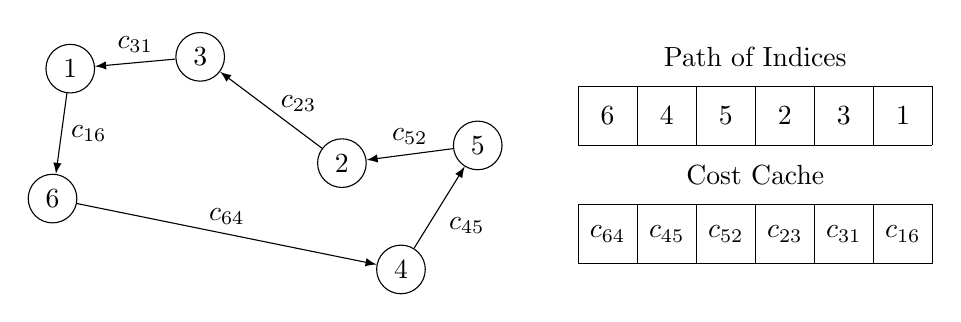
\begin{tikzpicture}[scale=0.75]
        \node[circle, draw, fill=white] (A) at (2.6, 4) {3};
        \node[circle, draw, fill=white] (B) at (0.4, 3.8) {1};
        \node[circle, draw, fill=white] (C) at (0.1, 1.6) {6};
        \node[circle, draw, fill=white] (D) at (6, 0.4) {4};
        \node[circle, draw, fill=white] (E) at (7.3, 2.5) {5};
        \node[circle, draw, fill=white] (F) at (5, 2.2) {2};
    
       \draw[-latex] (A) to node[above,] {$c_{31}$} (B);
		\draw[-latex] (B) to node[right] {$c_{16}$} (C);
		\draw[-latex] (C) to node[above] {$c_{64}$} (D);
		\draw[-latex] (D) to node[below right] {$c_{45}$} (E);
		\draw[-latex] (E) to node[above] {$c_{52}$} (F);
		\draw[-latex] (F) to node[above right, yshift=-4] {$c_{23}$} (A);
	
		\begin{scope}[shift={(9, 1.5)}]
			\draw (0,1) grid (6,2);
			\path (.5,.5) (0.5,1.5) node{$6$} ++(1,0) node{$4$} ++(1,0) node{$5$} ++(1,0) node{$2$} ++(1,0) node{$3$} ++(1,0) node{$1$};
			\draw (3,2.5) node{Path of Indices};
        \end{scope} 

		\begin{scope}[shift={(9, -0.5)}]
			\draw (0,1) grid (6,2);
			\path (.5,.5) (0.5,1.5) node{$c_{64}$} ++(1,0) node{$c_{45}$} ++(1,0) node{$c_{52}$} ++(1,0) node{$c_{23}$} ++(1,0) node{$c_{31}$} ++(1,0) node{$c_{16}$};
			\draw (3,2.5) node{Cost Cache};
        \end{scope}    

    \end{tikzpicture}
    \caption{Representation of the Cost-Cache.}
    \label{fig:solRepresentationExample}
\end{figure}

\begin{figure}[htbp]
    \centering
    \begin{tikzpicture}
        \begin{axis}[
            width=11cm, height=8cm,
            ymajorgrids=true,
            grid style={dashed,gray!30},
            xlabel=Instance size,
            ymin=1, ymax=1.5,
            ylabel=,
            legend style={at={(0.02,0.98)},anchor=north west,legend columns=-1},
            symbolic x coords={100,500,1000,5000,10000},
            log ticks with fixed point,
            xtick=data,
            ytick={1,1.1,1.2,1.3,1.4},
            yticklabels={0\%,10\%,20\%,30\%,40\%},
            ybar, 
                    ]
            \addplot[Blue,fill] table[x=n, y=cmpcc_base, col sep=semicolon] {csv/cmp_2opt.csv};
            \addplot[Red,fill] table[x=n, y=cmpcc_matrix, col sep=semicolon] {csv/cmp_2opt.csv};
            \addplot[Green,fill] table[x=n, y=cmpcc_avx_approx, col sep=semicolon] {csv/cmp_2opt.csv};
            \legend{Basic,Matrix,AVX}
        \end{axis}
    \end{tikzpicture}
    \caption{Speedup gained by each approach using the cost cache in 2-Opt.} \label{fig:costCacheShowcase} 
\end{figure}

\subsection{Solution Cost Precision}

Throughout the execution of any implemented algorithm, the overall cost of the solution being generated or optimized constantly changes.
During the project's development, we found it useful to update this value with each modification made to a solution.
Although this is a good practice for debugging the algorithms, it can sometimes lead to precision issues.
These issues stem from the limitations of floating-point standard representation.
For example, consider two numbers, $a=10^8$ and $b=1.53$.
When using the 32-bit floating-point standard, $a+b=10^8=a$, because the bits of the mantissa of $b$ are \textit{out of bounds} compared to those of $a$.
This situation can arise when a solution has been optimized, and its overall cost is the result of adding or subtracting minor improvements throughout the optimization process.
As a result, when the cost of the solution is recomputed at the end of the optimization procedure - usually to verify if it matches the current solution cost - these values might differ slightly. 
This is especially true for very large instances.

A solution to this problem is to store the cost of the solution in a higher precision variable.
Extending the variable to 64 bits resolved the issue for the most part, but did not completely eliminate it.

The best solution we found was to switch from floating-point to fixed-point representation.
Since fixed-point representation does not have a standard implementation in the C language, we implemented one ourselves.
We used 128 bits, with 64 for the integer part and the remaining 64 for the fractional part.
This effectively eliminated all the precision issues we encountered, although it's not without drawbacks: fixed-point variables are less flexible with large ranges compared to floating-point ones.

This precision problem is only a concern during debugging, as in production, it may be sufficient to simply recompute the cost of the solution when necessary.
